\subsection*{Problema 25}

\textbf{Enunciado:}
Calcular la integral indefinida:
\begin{align*}
\int x^4 \sqrt{1 - x^2} \, dx
\end{align*}

\textbf{Solución:}
Para resolver la integral, aplicamos la sustitución trigonométrica sugerida. Sea:
\begin{align*}
x &= \sin\theta \\
dx &= \cos\theta \, d\theta
\end{align*}

Sustituyendo en la integral y utilizando la identidad $\sqrt{1 - \sin^2\theta} = \cos\theta$:
\begin{align*}
I &= \int (\sin\theta)^4 (\cos\theta) (\cos\theta \, d\theta) \\
I &= \int \sin^4\theta \cos^2\theta \, d\theta
\end{align*}

Reescribimos la expresión usando potencias agrupadas:
\begin{align*}
I &= \int (\sin\theta \cos\theta)^2 \sin^2\theta \, d\theta \\
I &= \int \left(\dfrac{\sin(2\theta)}{2}\right)^2 \left(\dfrac{1 - \cos(2\theta)}{2}\right) d\theta
\end{align*}

Expandiendo la expresión constante:
\begin{align*}
I &= \dfrac{1}{8} \int \sin^2(2\theta) (1 - \cos(2\theta)) \, d\theta \\
I &= \dfrac{1}{8} \int \sin^2(2\theta) \, d\theta \\
&\quad - \dfrac{1}{8} \int \sin^2(2\theta) \cos(2\theta) \, d\theta
\end{align*}

Para la primera integral, usamos la identidad del ángulo medio $\sin^2(\alpha) = \frac{1 - \cos(2\alpha)}{2}$:
\begin{align*}
\int \sin^2(2\theta) \, d\theta &= \int \dfrac{1 - \cos(4\theta)}{2} \, d\theta \\
&= \dfrac{\theta}{2} - \dfrac{\sin(4\theta)}{8}
\end{align*}

Para la segunda integral, aplicamos sustitución directa con $u = \sin(2\theta)$:
\begin{align*}
\int \sin^2(2\theta) \cos(2\theta) \, d\theta = \dfrac{\sin^3(2\theta)}{6}
\end{align*}

Combinando ambos resultados y multiplicando por el factor $\frac{1}{8}$:
\begin{align*}
I &= \dfrac{\theta}{16} - \dfrac{\sin(4\theta)}{64} - \dfrac{\sin^3(2\theta)}{48} + C
\end{align*}

Utilizamos identidades de ángulo doble para regresar a la variable $\theta$:
\begin{align*}
\sin(4\theta) &= 2\sin(2\theta)\cos(2\theta) \\
&= 4\sin\theta\cos\theta(1 - 2\sin^2\theta)
\end{align*}

Sustituyendo $x = \sin\theta$ y $\cos\theta = \sqrt{1 - x^2}$:
\begin{align*}
\theta &= \arcsin(x) \\
\sin(2\theta) &= 2x\sqrt{1 - x^2}
\end{align*}

Sustituyendo de regreso en términos de $x$:
\begin{align*}
I &= \dfrac{\arcsin(x)}{16} \\
&\quad - \dfrac{x\sqrt{1-x^2}(1 - 2x^2)}{16} \\
&\quad - \dfrac{x^3(1-x^2)^{3/2}}{6} + C
\end{align*}

Simplificando los términos algebraicos, obtenemos la solución final:
\begin{align*}
I &= \dfrac{1}{16}\arcsin(x) \\
&\quad + \dfrac{x\sqrt{1-x^2}}{48} (2x^4 - x^2 - 2) + C
\end{align*}

\begin{figure}[H]
	\centering
	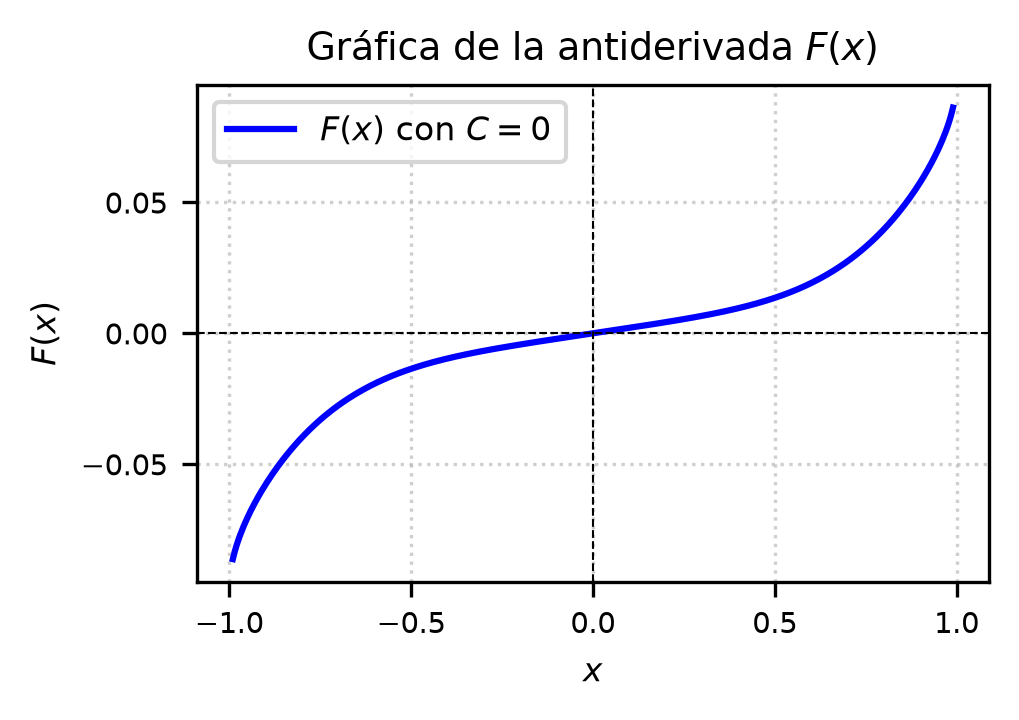
\includegraphics[width=\columnwidth]{semana_05/graficas/SEM05_P25_grafica.png}
	\caption{Representación gráfica de $f(x)$ y su antiderivada $F(x)$ evaluada para la constante de integración $C = 0$ (Problema 25).}
	\label{fig:problema25}
\end{figure}
